\documentclass[a4paper,10pt]{article}
\usepackage[left=2cm,top=3cm,right=3cm,bottom=3cm]{geometry}
\usepackage{enumerate}
\usepackage{multicol}
\usepackage{verbatim}
\usepackage{amssymb,amsmath} 
\usepackage{amsthm}
\usepackage[pdftex]{graphicx}
\usepackage{listings}
\newcommand{\code}[1]{\texttt{#1}}
\newcommand{\figref}[1]{(fig. \ref{#1})}
%\bibliographystyle{prsty} % Choose Phys. Rev. stylle for bibliography
\bibliographystyle{plain}


\lstset{language=C,basicstyle=\small,frame=single,showstringspaces=false,breaklines=true,breakatwhitespace=true}
\begin{document}
\title{\textbf{Project}:\\Netfilter/iptables}
\author{Andrew Rimes - cs253030\\Kreshnik Mati - cse93062\\CSE4221 - F09}
\date{December 8, 2009}

\maketitle
\thispagestyle{empty} 

\newpage

\setcounter{tocdepth}{3}
\tableofcontents


\newpage

\section{Overview}


\begin{figure}
\centering
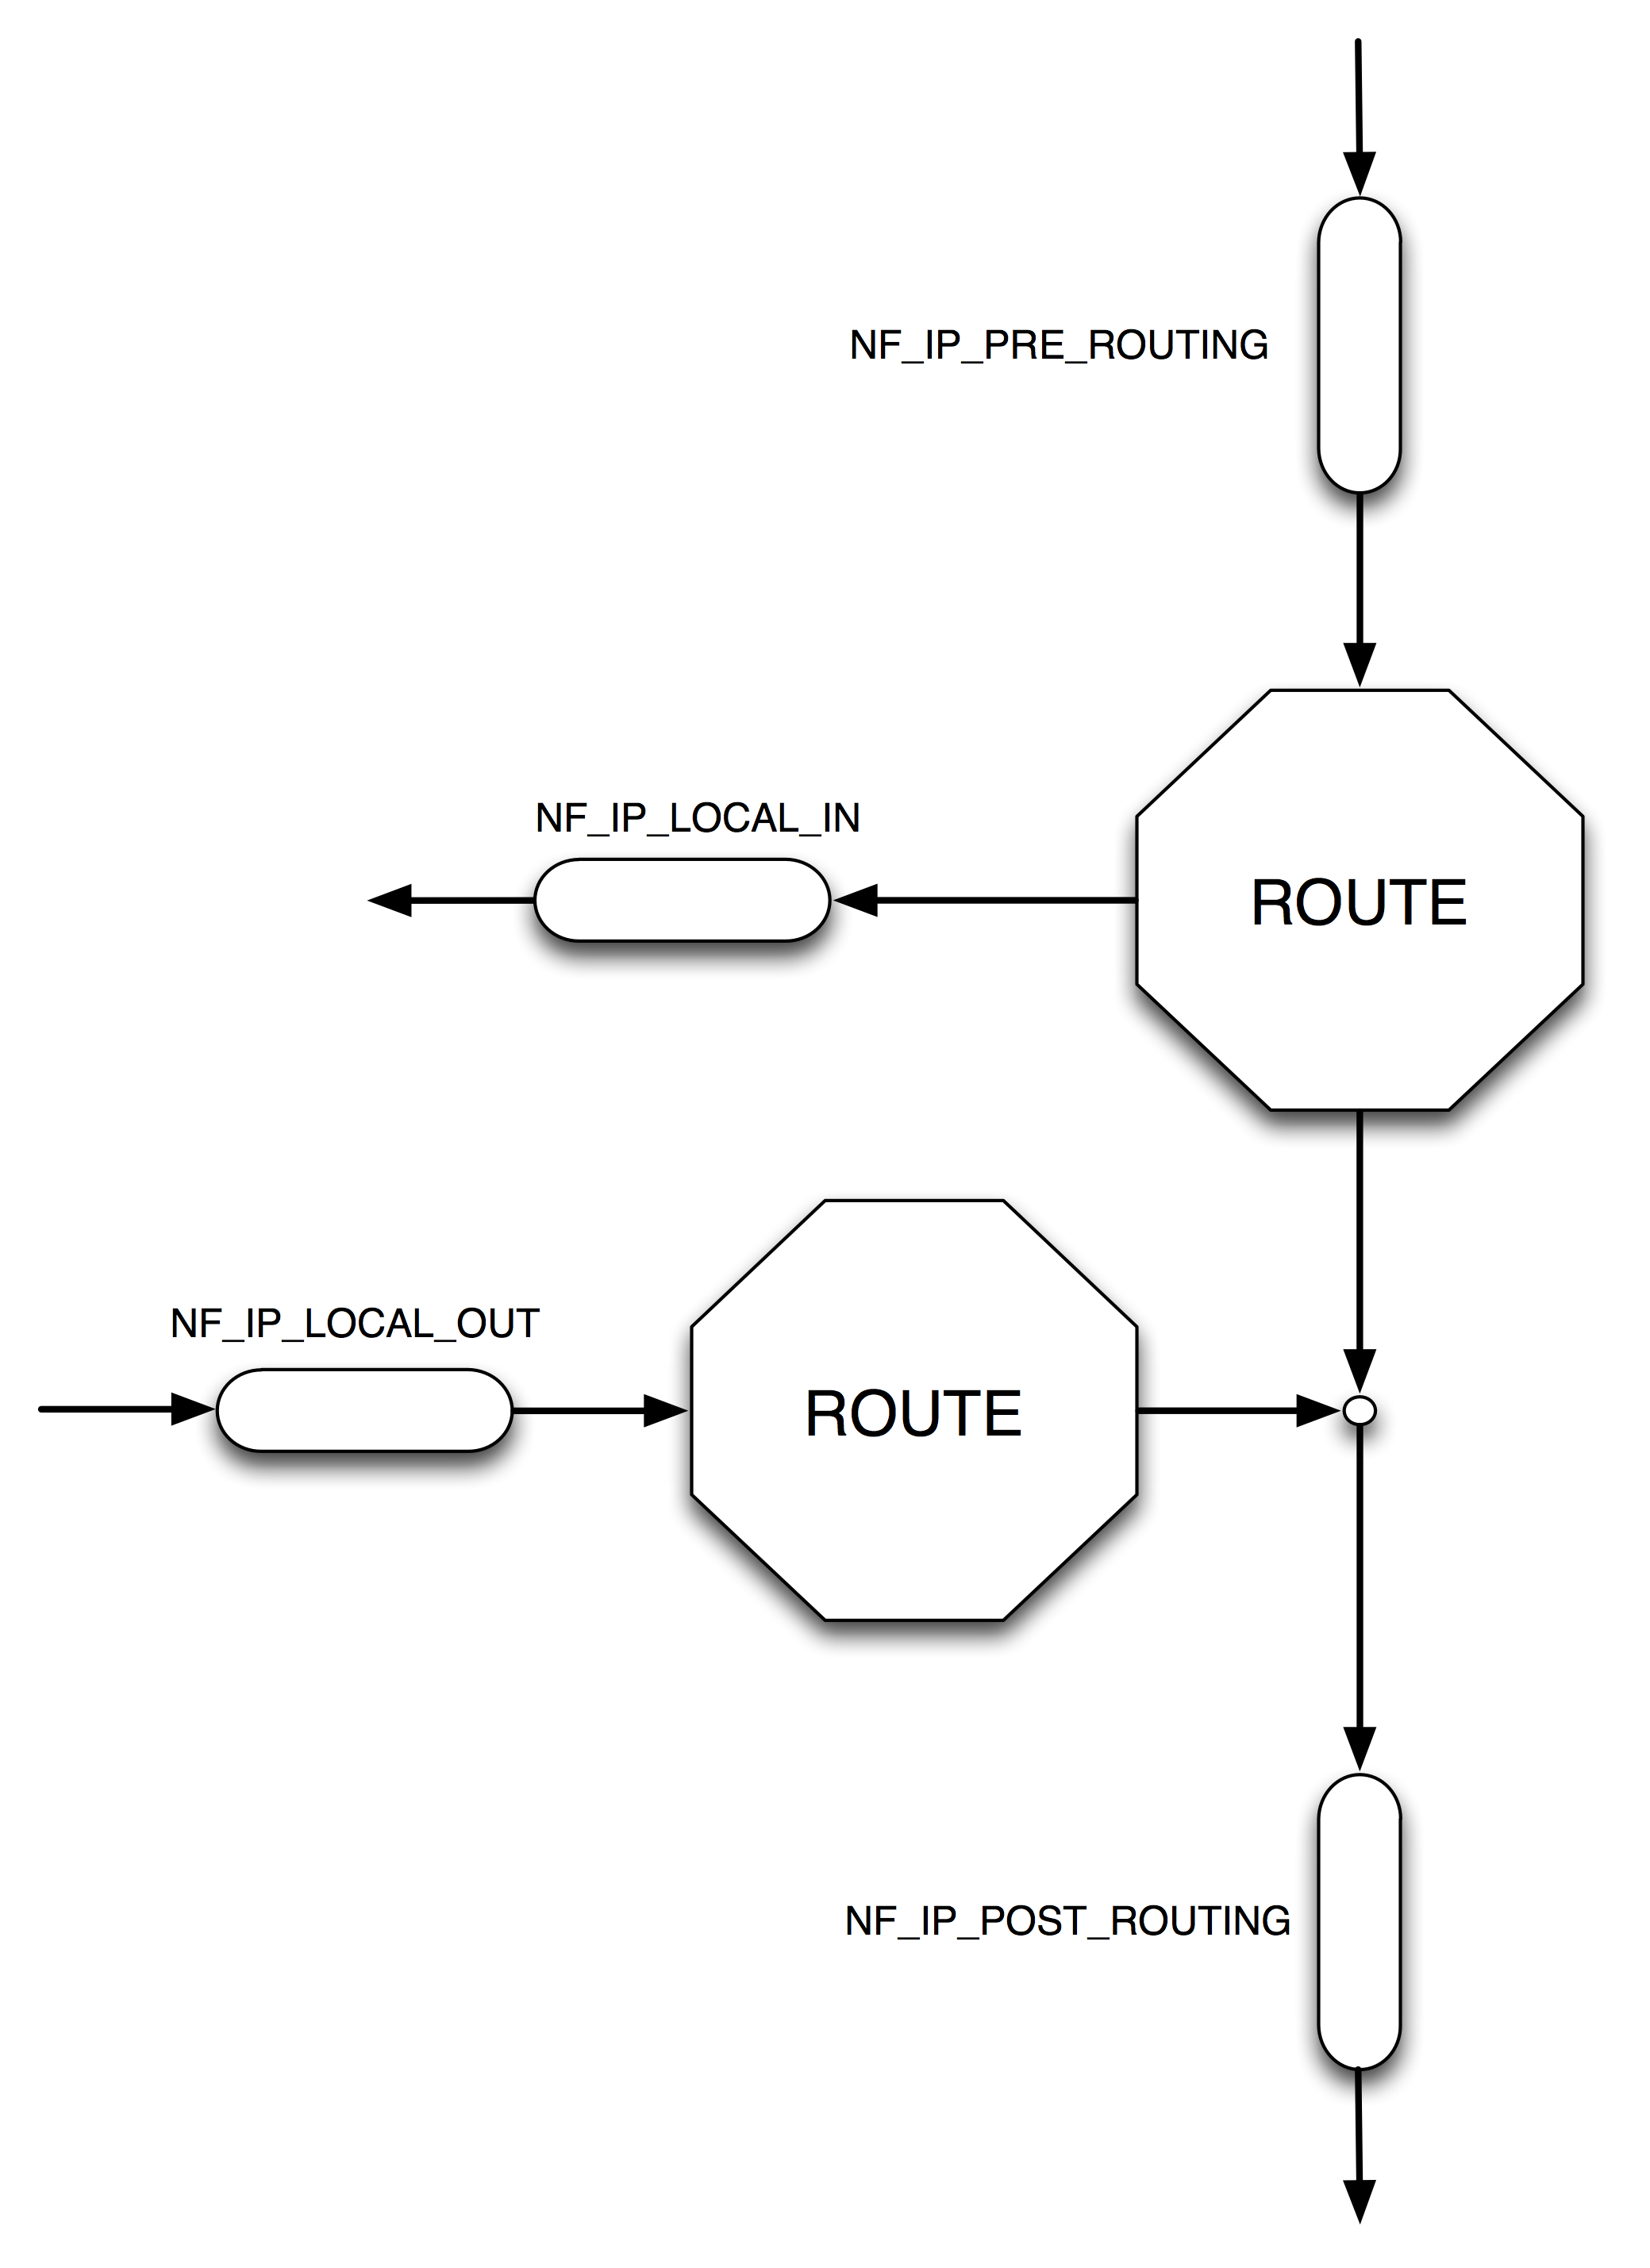
\includegraphics[totalheight=0.40\textheight]{images/hooks.png}
\caption{The packet is passed into \code{iptables}' hooks at certain points
  before and after routing.}\label{fig:hooks}
\end{figure}

\section{Data Structures}
  

\subsection{ip\_tables.h}

An IP table is made of multiple chains; a chain is a list of
rules. Each rule consists of one or more matches, terminated by a
target. The target is the action performed when a rule is entirely
matched. The userspace tool \code{iptables} is used to manipulate the IP
tables. The data structures are designed such that they can be used in
both user and kernel mode.

\subsubsection{ipt\_ip}\label{ipt_ip}

This struct specifies the minimal IP header information needed
to to identify a packet. The \code{src} and \code{dst} fields identify
the source and destination IP addresses, and \code{smsk} and
\code{dmsk} identify the source and destination masks so that ranges
of IP addresses can be specified in the rule, e.g. 192.168.0.0/24
would match all IPs in the 192.168.0.0 subnet. The \code{initface} and
\code{outiface} fields specify inbound and outbound interfaces, and
\code{iniface\_mask} and \code{outiface\_mask} allow the user to specify several
interfaces at once. The protocol number is stored in \code{proto},
e.g. it would be set to 6 for TCP. The fields \code{flags} and
\code{invflags} specified the IP header flags selected and not selected.

\begin{lstlisting}

struct ipt_ip {
	/* Source and destination IP addr */
	struct in_addr src, dst;
        /* Mask for src and dest IP addr */
        struct in_addr smsk, dmsk;
        char iniface[IFNAMSIZ], outiface[IFNAMSIZ];
        unsigned char iniface_mask[IFNAMSIZ], outiface_mask[IFNAMSIZ];

        /* Protocol, 0 = ANY */
        u_int16_t proto;

        /* Flags word */
        u_int8_t flags;
        /* Inverse flags */
        u_int8_t invflags;
};

\end{lstlisting}

\subsubsection{ipt\_entry}

This structure defines the starting point of each of the firewall
rules, which are contained in arrays, i.e. tables.  The
\code{nf\_cache} bitfield shows what parts of the packet this rule
exams. The \code{target\_offset} field indicates the offset between
the beginning of the current rule (contained in the structure) and
where the \code{ipt\_entry\_target} begins. As indicated in the
comments, the target offset is equal to the size of the
\code{ipt\_entry} and the total number of matches. The
\code{next\_offset} is the sum of the entry, matches, and target,
which determines the position of the next rule's
\code{ipt\_entry}. The target, described elsewhere, is executed when
the rule matches. The \code{comefrom} field is a back pointer used by
the kernel to track packet traversal. Obviously, \code{counters}
stores packet and byte counts for the rule, i.e. how many have passed
through. The final, variable length field \code{elems} is where matches,
terminated by the target, are stored.

\begin{lstlisting}
struct ipt_entry
{
        struct ipt_ip ip;

        /* Mark with fields that we care about. */
        unsigned int nfcache;

        /* Size of ipt_entry + matches */
        u_int16_t target_offset;
        /* Size of ipt_entry + matches + target */
        u_int16_t next_offset;

        /* Back pointer */
        unsigned int comefrom;

        /* Packet and byte counters. */
        struct xt_counters counters;

        /* The matches (if any), then the target. */
        unsigned char elems[0];
};
\end{lstlisting}

\subsection{x\_tables.h}

\subsubsection{xt\_entry\_match (ipt\_entry\_match)}

This provides a thin layer of abstraction so that code can be reused
regardless of whether it is executing in the kernel or in user
space. We will discuss \code{xt\_match} since we are concerned with
the kernel\footnote{In some cases, structs have two names: one begining with xt and one
without. This is a result of the unification of common code in
\code{ip\_tables}, \code{ip6\_tables} and \code{arp\_tables} into \code{x\_tables} (hence xt) -- a table
structure that can handle all three protocols.}.

\begin{lstlisting}
struct xt_entry_match
{
        union {
                struct {
                        __u16 match_size;

			/* Used by userspace */
                        char name[XT_FUNCTION_MAXNAMELEN-1];

                        __u8 revision;
                } user;
		struct {
                        __u16 match_size;

                        /* Used inside the kernel */
                        struct xt_match *match;
                } kernel;

                /* Total length */
                __u16 match_size;
        } u;

        unsigned char data[0];
};
\end{lstlisting}

\subsubsection{xt\_match}\label{xt_match}
This structure represents a match entry in a rule (possibly one of
many). It is fairly abstract and meant to represent all types of
matches.

The \code{list} is the standard doubly linked list used in
the Linux kernel; this simple struct has two fields, \code{prev} and
\code{nest}, and  is defined in \code{include/linux/list.h}. In this
case it is used to link together consecutive matches in the rule
[maybe?? guess]. The \code{name} field stores the name of the current
callback function [?? verify]. The \code{revision} field stores the
current revision number of the data structure so that if it changes in
the future, backwards compatibility can be maintained.

The \code{match} field is a pointer to the boolean function that
determines whether or not the packet will be matched. The \code{skb}
parameter is a pointer to a copy of the packet and
\code{xt\_match\_param} is a pointer to additional parameters the
match function can use to make the decision.

The function pointed to by \code{checkentry} is called when the user
attempts to add this type of match to the rule (whatever that type is). The struct
\code{xt\_mtchk\_param} (\ref{xt_mtchk_param}) is passed to make that decision. 

\begin{lstlisting}
struct xt_match
{
        struct list_head list;

        const char name[XT_FUNCTION_MAXNAMELEN-1];
        u_int8_t revision;

        /* Return true or false: return FALSE and set *hotdrop = 1 to                                                                                       
           force immediate packet drop. */
       bool (*match)(const struct sk_buff *skb,
                      const struct xt_match_param *);

        /* Called when user tries to insert an entry of this type. */
        bool (*checkentry)(const struct xt_mtchk_param *);

        /* Called when entry of this type deleted. */
        void (*destroy)(const struct xt_mtdtor_param *);

        /* Called when userspace align differs from kernel space one */
        void (*compat_from_user)(void *dst, void *src);
        int (*compat_to_user)(void __user *dst, void *src);

        /* Set this to THIS_MODULE if you are a module, otherwise NULL */
        struct module *me;

        /* Free to use by each match */
        unsigned long data;

        const char *table;
        unsigned int matchsize;
        unsigned int compatsize;
        unsigned int hooks;
        unsigned short proto;

        unsigned short family;
};
        
\end{lstlisting}

\subsubsection{xt\_mtchk\_param}\label{xt_mtchk_param}

This struct is passed to a match extesion's \code{checkentry}
function. The name of the table is in \code{table}. Protocol family
information, (e.g. \code{ipt\_ip} (\ref{ipt_ip}) for IPv4) is stored
in \code{entryinfo}.  The pointer \code{match} is the \code{xt\_match}
through which this function was invoked. The protocol family number is
stored in \code{family}.  Which hooks the new rule is reachable from
is stored in \code{hook\_mask} where each hook is defined by a
bit. Any additional information is stored in \code{matchinfo}.

\begin{lstlisting}
struct xt_mtchk_param {
        const char *table;
        const void *entryinfo;
	const struct xt_match *match;
        void *matchinfo;
	unsigned int hook_mask;
	u_int8_t family;
};
\end{lstlisting}

\subsubsection{xt\_target (ipt\_entry\_target)}

This structure represents the final target entry in a rule and is
analogous to \code{xt\_match} (\ref{xt_match}). Just as
\code{xt\_match} has a pointer to a match and checkentry functions,
\code{xt\_target} has pointers to a \code{target} function and its own
\code{checkentry} function. Similarly, it has to deal with possible
differences in memory alignment between kernel and user space. The
\code{me} pointer is used to identify the entry within modules.

\begin{lstlisting}
struct xt_target
{
        struct list_head list;

        const char name[XT_FUNCTION_MAXNAMELEN-1];

        /* Returns verdict. Argument order changed since 2.6.9, as this                                                                                     
           must now handle non-linear skbs, using skb_copy_bits and                                                                                         
           skb_ip_make_writable. */
        unsigned int (*target)(struct sk_buff *skb,
                               const struct xt_target_param *);

        /* Called when user tries to insert an entry of this type:                                                                                          
           hook_mask is a bitmask of hooks from which it can be                                                                                             
           called. */
        /* Should return true or false. */
        bool (*checkentry)(const struct xt_tgchk_param *);

        /* Called when entry of this type deleted. */
        void (*destroy)(const struct xt_tgdtor_param *);

        /* Called when userspace align differs from kernel space one */
        void (*compat_from_user)(void *dst, void *src);
        int (*compat_to_user)(void __user *dst, void *src);

        /* Set this to THIS_MODULE if you are a module, otherwise NULL */
        struct module *me;

        const char *table;
        unsigned int targetsize;
        unsigned int compatsize;
        unsigned int hooks;
        unsigned short proto;

        unsigned short family;
        u_int8_t revision;
};
\end{lstlisting}

\subsection{Diagrams}

\begin{figure}[H]
\centering
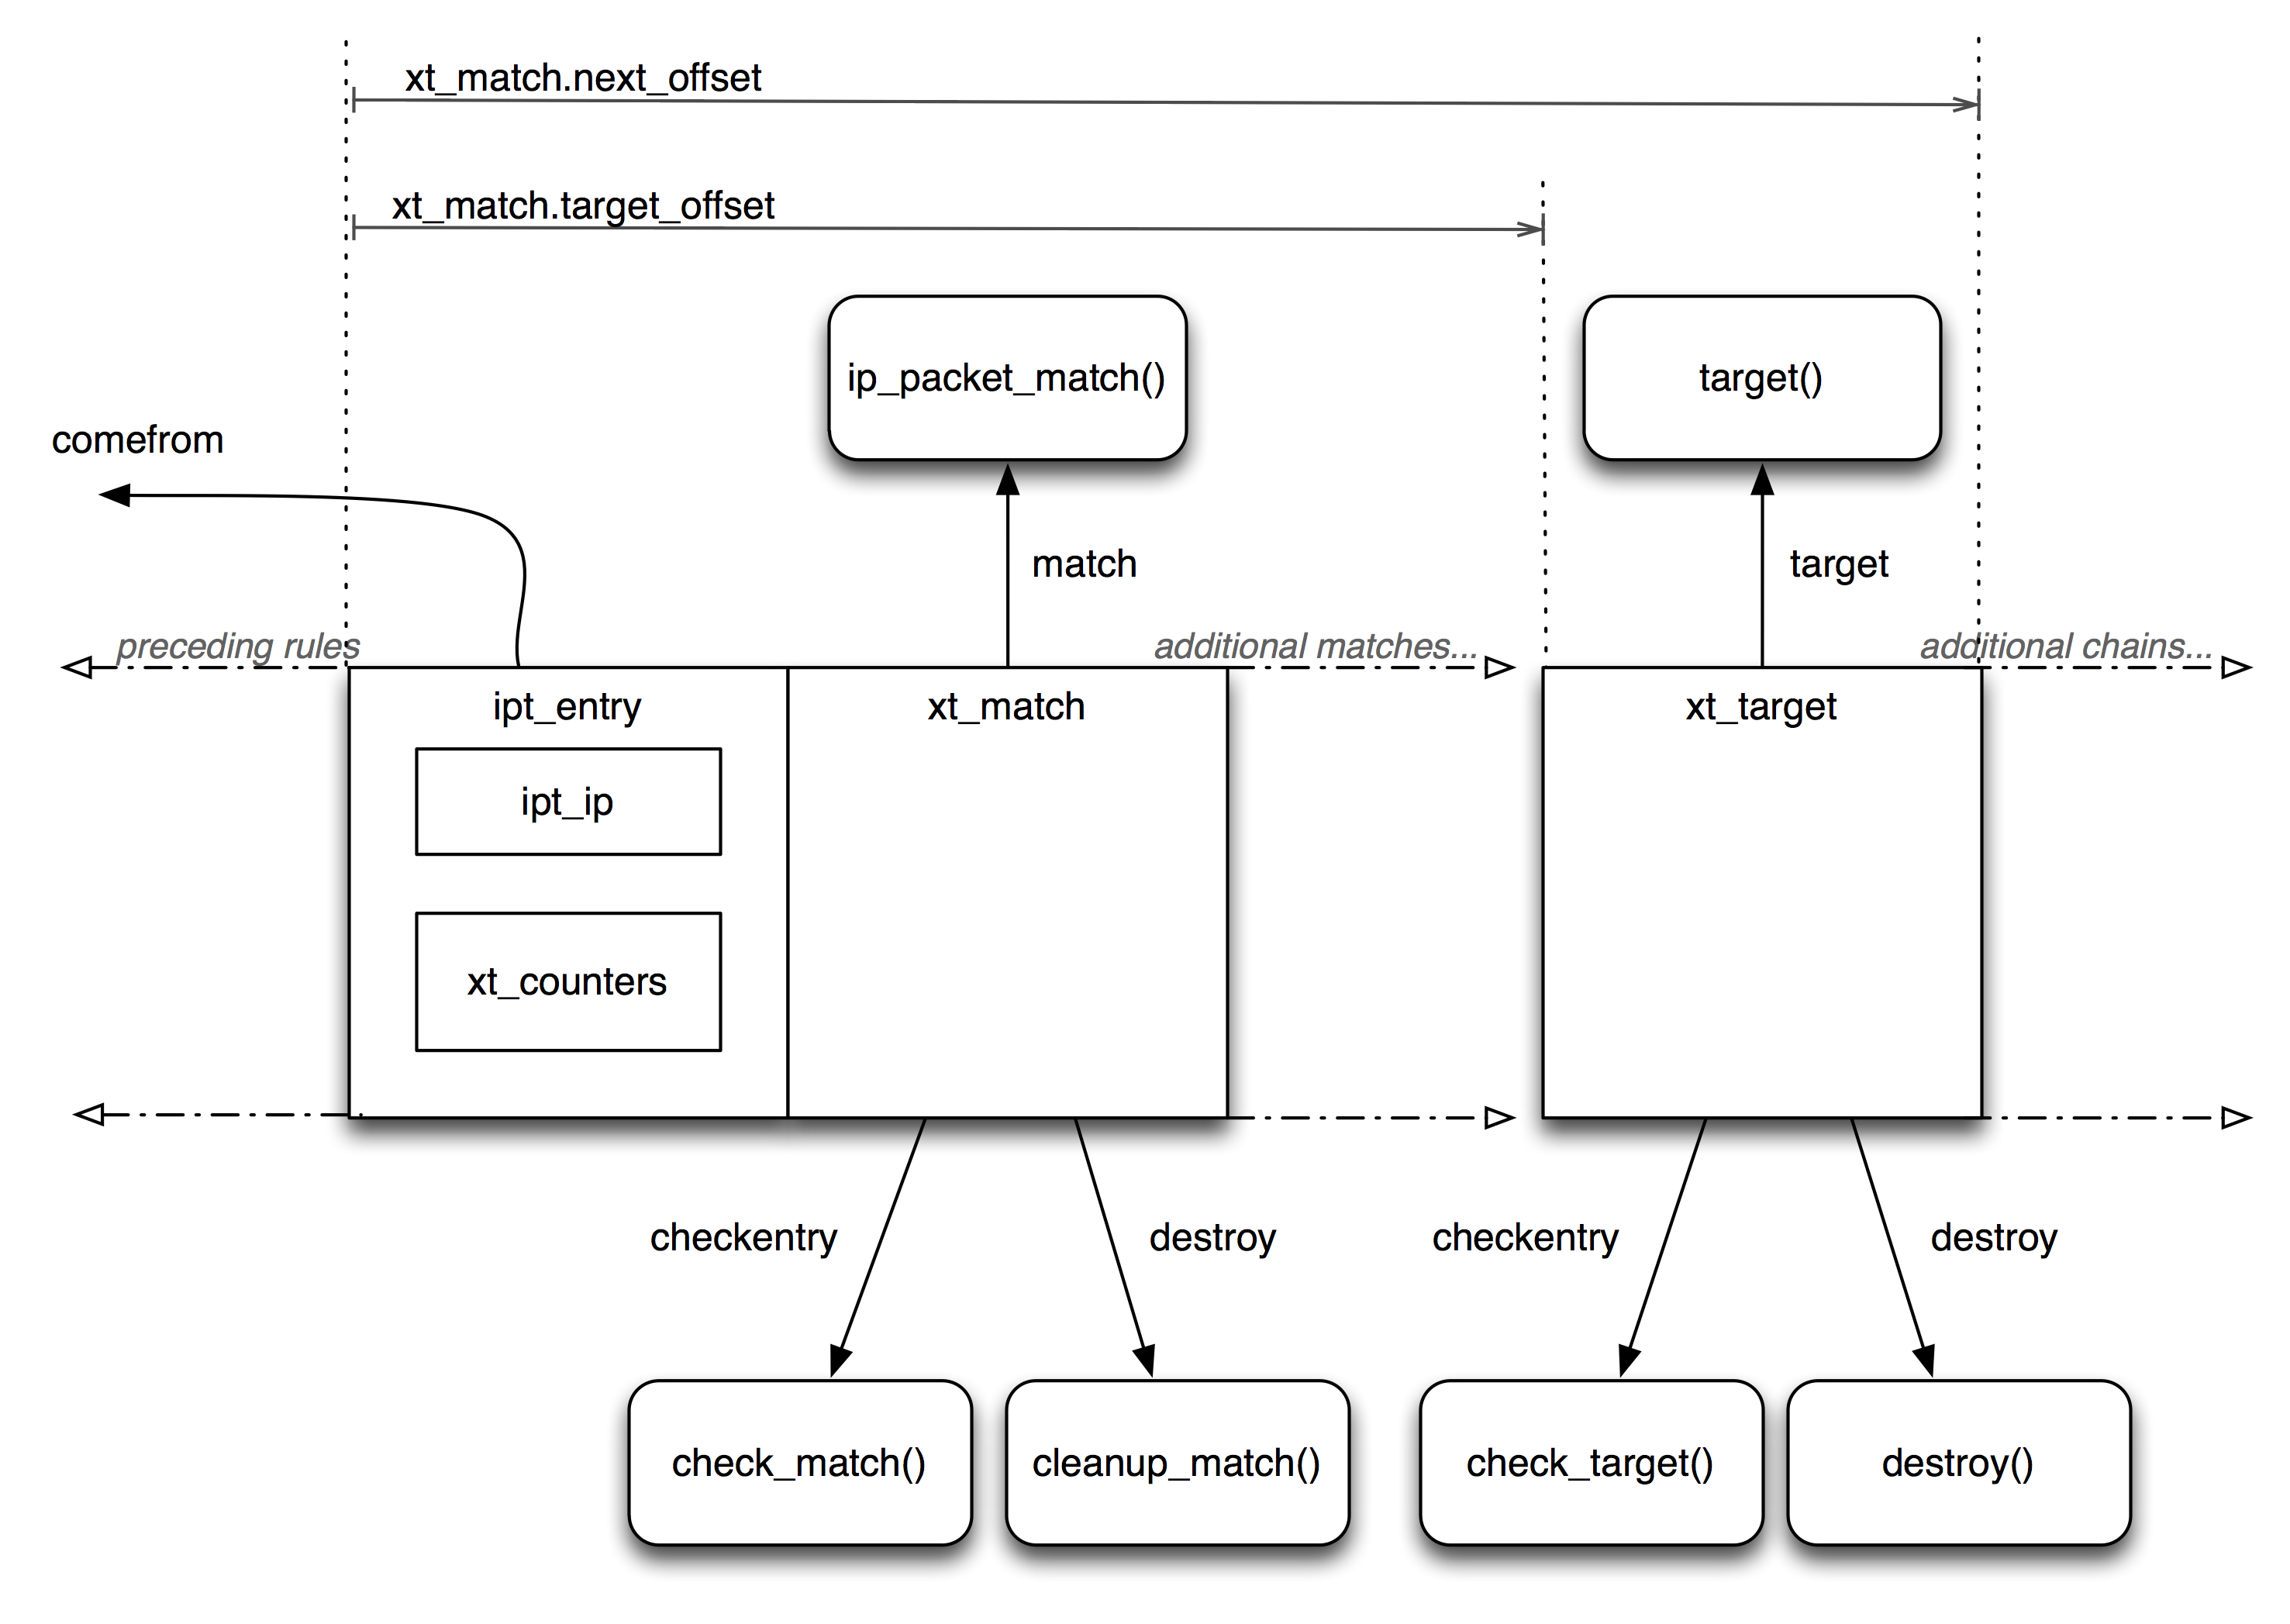
\includegraphics[totalheight=0.45\textheight]{images/table1.png}
\caption{The structure of an \code{iptables} IPv4 table.}\label{fig:table1}
\end{figure}

\section{Execution}

\subsection{ip\_tables.h}

For historical reasons, the IP specific \code{IPT\_MATCH\_ITERATE}
macro calls the more general \code{XT\_MATCH\_ITERATE}. 

\begin{lstlisting}
  /* fn returns 0 to continue iteration */
#define IPT_MATCH_ITERATE(e, fn, args...) \
	XT_MATCH_ITERATE(struct ipt_entry, e, fn, ## args)
\end{lstlisting}

Similarly, the IPv4 specific \code{IPT\_ENTRY\_ITERATRE} calls
\code{XT\_ENTRY\_ITERATE} to iterate through the rule entries begining
at \code{ipt\_entry}.

\begin{lstlisting}
  /* fn returns 0 to continue iteration */
#define IPT_ENTRY_ITERATE(entries, size, fn, args...) \
	XT_ENTRY_ITERATE(struct ipt_entry, entries, size, fn, ## args)
\end{lstlisting}

\subsection{x\_tables.h}

\subsubsection{XT\_MATCH\_ITERATE}

The \code{XT\_MATCH\_ITERATE} macro expands to a for loop that
iterates through the list of \code{xt\_match} structures starting from
the \code{ipt\_entry}. With each step, the index into the rule is
advanced by the length of the current \code{xp\_match} object and the
associated match function is called. If the match functions returns 0, i.e. the packet
matches, the iteration continues.


\begin{lstlisting}
/* fn returns 0 to continue iteration */
#define XT_MATCH_ITERATE(type, e, fn, args...)			\
({								\
	unsigned int __i;					\
	int __ret = 0;						\
	struct xt_entry_match *__m;				\
								\
	for (__i = sizeof(type);				\
	     __i < (e)->target_offset;				\
	     __i += __m->u.match_size) {			\
		__m = (void *)e + __i;				\
								\
		__ret = fn(__m , ## args);			\
		if (__ret != 0)					\
			break;					\
	}							\
	__ret;							\
})

\end{lstlisting}


\subsubsection{XT\_ENTRY\_ITERATE\_CONTINUE and XT\_ENTRY\_ITERATE}

The \code{XT\_ENTRY\_ITERATE\_CONTINUE} and \code{XT\_ENTRY\_ITERATE}
macros are used whenever it is necessary to walk through a table
applying the function \code{fn} on each
entry\footnote{\code{XT\_ENTRY\_ITERATE} skips the application of
  \code{fn} on the first entry.}.

\begin{lstlisting}
/* fn returns 0 to continue iteration */
#define XT_ENTRY_ITERATE(type, entries, size, fn, args...) \
	XT_ENTRY_ITERATE_CONTINUE(type, entries, size, 0, fn, args)

/* fn returns 0 to continue iteration */
#define XT_ENTRY_ITERATE_CONTINUE(type, entries, size, n, fn, args...) \
({								\
	unsigned int __i, __n;					\
	int __ret = 0;						\
	type *__entry;						\
								\
	for (__i = 0, __n = 0; __i < (size);			\
	     __i += __entry->next_offset, __n++) { 		\
		__entry = (void *)(entries) + __i;		\
		if (__n < n)					\
			continue;				\
								\
		__ret = fn(__entry , ## args);			\
		if (__ret != 0)					\
			break;					\
	}							\
	__ret;							\
})
\end{lstlisting}

\subsection{ip\_tables.c}

\subsubsection{ip\_packet\_match}

Below is the basic match function that is performed on the header of
every incoming packet (with some debugging statements omitted). Lines
12-17 apply the netmask from the rule to the source and destination
IPs of the packet header \code{iphdr} and verifies that they
correspond to the fields in \code{ipt\_ip}(\ref{ipt_ip}). It also
verifies that the rule is checking source and destination
addresses. Lines 19-29 verify that the incoming and outgoing interface
of the packet correspond to the rule and that the rule checks for
interfaces. Lines 31-35 verify the protocol matches and that the
protocol is being checked. The final check on line 39 verifies that if
the match applies to fragmented packets, that the packet is
fragmented.


\lstset{stepnumber=1,frame=single,numbers=left,numberstyle=\footnotesize}

\begin{lstlisting}
static inline bool
ip_packet_match(const struct iphdr *ip,
		const char *indev,
		const char *outdev,
		const struct ipt_ip *ipinfo,
		int isfrag)
{
	unsigned long ret;

#define FWINV(bool, invflg) ((bool) ^ !!(ipinfo->invflags & (invflg)))

	if (FWINV((ip->saddr&ipinfo->smsk.s_addr) != ipinfo->src.s_addr,
		  IPT_INV_SRCIP)
	    || FWINV((ip->daddr&ipinfo->dmsk.s_addr) != ipinfo->dst.s_addr,
		     IPT_INV_DSTIP)) {
		return false;
	}

	ret = ifname_compare_aligned(indev, ipinfo->iniface, ipinfo->iniface_mask);

	if (FWINV(ret != 0, IPT_INV_VIA_IN)) {
		return false;
	}

	ret = ifname_compare_aligned(outdev, ipinfo->outiface, ipinfo->outiface_mask);

	if (FWINV(ret != 0, IPT_INV_VIA_OUT)) {
		return false;
	}

	/* Check specific protocol */
	if (ipinfo->proto
	    && FWINV(ip->protocol != ipinfo->proto, IPT_INV_PROTO)) {
		return false;
	}

	/* If we have a fragment rule but the packet is not a fragment
	 * then we return zero */
	if (FWINV((ipinfo->flags&IPT_F_FRAG) && !isfrag, IPT_INV_FRAG)) {
		return false;
	}

	return true;
}
\end{lstlisting}

The \code{do\_match} function is the function called by the
\code{XT\_MATCH\_ITERATOR} macro. It executes the match routine
associted with each match entry in the rule, for example it would call
\code{ip\_packet\_match} above for a basic IPv4 match.

\lstset{stepnumber=0}
\begin{lstlisting}
 static inline bool
do_match(struct ipt_entry_match *m, const struct sk_buff *skb,
	 struct xt_match_param *par)
{
	par->match     = m->u.kernel.match;
	par->matchinfo = m->data;

	/* Stop iteration if it doesn't match */
	if (!m->u.kernel.match->match(skb, par))
		return true;
	else
		return false;
}
\end{lstlisting}

\end{document}